\documentclass[12pt,a4paper]{article}
\usepackage[utf8]{inputenc}
\usepackage[english]{babel}
\usepackage{amsmath}
\usepackage{amsfonts}
\usepackage{amssymb}
\usepackage{graphicx}
\usepackage{tabularx}
\usepackage{url}
\usepackage{float}
\usepackage{color} 
\usepackage[sort=use]{glossaries-extra}

%\definecolor{pagecolor}{rgb}{0.8,0.9,0.9}

\usepackage[tocflat]{tocstyle}
\usetocstyle{standard}

%MVP, EWASM, TPS, ABCI, SDK, WebAssembly, DAO, DEPOT, ZK, PoS, Plasma

\newglossaryentry{evm}{name={EVM},plural={EVMs},
description={Ethereum Virtual Machine is designed to serve as a runtime environment for smart contracts based on Ethereum.}}
\newglossaryentry{blockchain}{name={Blockchain},plural={Blockchains},
description={A system in which a record of transactions are maintained across several computers that are linked in a peer-to-peer network.}}
\newglossaryentry{ethereum}{name={Ethereum},plural={Ethereum},
description={A decentralized software platform that enables SmartContracts and Distributed Applications (ĐApps).}}
\newglossaryentry{eth}{name={ETH},plural={eth},
description={Native token of the Ethereum blockchain.}}
\newglossaryentry{btc}{name={BTC},plural={BTC},
description={Native token of the Bitcoin blockchain.}}
\newglossaryentry{erc20}{name={ERC20},plural={ERC20},
description={A technical standard used for smart contracts on the Ethereum blockchain for implementing tokens.}}
\newglossaryentry{smartcontract}{name={SmartContract},plural={SmartContract},
description={A smart contract is a computer protocol intended to digitally facilitate, verify, or enforce the negotiation or performance of a contract. Smart contracts allow the performance of credible transactions without third parties. These transactions are trackable and irreversible.}}
\newglossaryentry{account}{name={Account},plural={accounts},
description={A hash of a public key which can hold values. Hold values can only be accessed by knowing the corresponding private key.}}
\newglossaryentry{gdpr}{name={GDPR},plural={GDPR},
description={The General Data Protection Regulation (EU) 2016/679 ("GDPR") is a regulation in EU law on data protection and privacy for all individuals within the European Union (EU).}}
\newglossaryentry{payg}{name={PAYG},plural={PAYG},
description={a method of financing social insurance, especially old-age provision, but also health insurance and unemployment insurance. The paid-in contributions are used directly to finance the beneficiaries, ie they are paid back to them.}}


\begin{document}

%\pagecolor{pagecolor}
\pagenumbering{gobble}% Remove page numbers (and reset to 1)
\clearpage

% NEW SITE ---------------------------------------------------------------------------------
\begin{figure}
    \centering
    
\includegraphics[width=2.0in]{logo.png}
\end{figure}

\title{ASURE: An open-source, SCALABLE BLOCKCHAIN NETWORK FOR DECENTRALIZED SOCIAL SECURITY SYSTEMS}
\author{Paul Mizel, Fabian Raetz, Gamal Schmuck}
\date{September 19, 2018}
\maketitle

\vskip 2in

\begin{quote}
	\centering
	\url{http://asure.network}
\end{quote}

\newpage 
% NEW SITE ---------------------------------------------------------------------------------

\pagenumbering{arabic}% Arabic page numbers (and reset to 1)
\newpage

\begin{abstract}

Die Asure Stiftung hat sich das Ziel gesetzt, die Sozialversicherungssysteme dieser Welt mit Hilfe der neusten Technologien wie Blockchain zu erforschen und zu verbessern. 
Um die Herausforderungen und die Anforderungen zur Modernisierung und Entwicklung von umlagebasierten Systemen besser verstehen zu können, wurde der Prototyp des deutschen Rentensystems auf der öffentlichen Ethereum Blockchain entwickelt.
In diesem Dokument stellen wir das Ergebnis sowie die im Rahmen der Entwicklung gewonnenen Erkenntnisse vor.

\end{abstract}

\keywords{Blockchain, Ethereum, Sozialversicherung, Rentensystem, Deutsche Rentenversicherung, Umlageverfahren}



% list all entries
\printunsrtglossaries
\newpage
\tableofcontents

\newpage
% NEW SITE ---------------------------------------------------------------------------------
\section{Introduction}

Development over the last 150 years have led to a shift in old-age provision from the family association to larger groups (state, collective of the insured community). Pension systems today are an essential part of the economic development of states and yet, there are 4.1 billion people without access to social security.\cite{noauthor_universal_2017}

There are a variety of pension systems. For instance, in Germany pension systems are categorized into the three pillars of old-age provision. The three pillars include statutory, occupational and private pension systems. Many countries use a similar classification. As a general rule, the more pension systems a person participates in, the better he/she is protected against old-age poverty due to risk diversification.

\paragraph{Financing.} Occupational and private pension systems finance themselves through the funding method and generally follow the performance principle: those who contribute a lot to the pension system also get paid a lot when they get old.

Statutory pension systems finance themselves through the funding method, the pay-as-you-go method or a hybrid of the funding and the pay-as-you-go methods. In addition to the performance principle, many statutory pension insurance policies also follow the principle of solidarity. In Germany, for example, parental leave can be counted as contribution years in pension insurance.

Both the funding method and the pay-as-you-go method have proven their worth in the past. Both financing methods have their strengths and weaknesses, and opinions differ widely as to which financing method is the better one.
%Die Dezentrale Rente soll nach dem Vorbild der %Dezentralisierten Autonomen Organisation (DAO) von der %Community für die Community existieren und mehrere  Probleme %von heute vorhandenen Systeme beheben.

\subsection{Challenges of old-age provision}

Good old-age provision is hard to build. In the following we will discuss some of the challenges of old-age provision and existing pension systems.

\paragraph{Demographic change.} Life expectancy is increasing all over the world, and especially in industrialized nations, the proportion of people over the age of 60 is growing and the problem of retirement provision is becoming more pressing. The burden on pension systems, and in particular PAYG-funded pension schemes, is rising sharply as fewer contributors become available to provide pension payments. The population of developing countries will increase in the future, and thus the problem of retirement provision. For example, the United Nations estimates that by 2050, approximately two billion people will be over 60 years of age, of which as many as 80\% live in developing countries
\cite{noauthor_pensions_2009}.


\paragraph{Inflation.}  In economics, inflation refers to a general and sustained increase in the price level of goods and services (inflation), equivalent to a reduction in the purchasing power of money. The consumer price index (CPR) is most frequently used to measure inflation. The index is calculated with the help of a shopping basket, which is determined in a certain year (base year) representative of an average household. \cite{inflation} 
At an inflation rate of 2\%, this means from \$ 1,000 today, which in 2040 has only a purchasing power of \$ 672.97 in 2040. 
For this reason, it is important not to store the values, but to try to systematically preserve purchasing power by means of a pay-as-you-go system.

\paragraph{Mismanagement and fees.} Compared to pay-as-you-go systems, funded systems are very strongly subject to inflation. For this reason, different investment options are used, these have a higher workload and resulting administrative costs the customer must bear. Another variable is the higher volatility, it increases the chance that the investments are made well as well as the risk that bad investments can be made.

%\paragraph{Entertainment.} Todo:Die jeweils aktive und leistungsfähige Generation betreibt private Altersvorsorge und beteiligt sich zusätzlich ...
%The active and efficient generation in each case operates private old-age provision and also participates ...
%State-organized pension schemes, unlike privately-organized pension schemes, can use both the funded and the pay-as-you-go method.
%The state makes the guarantees and promises to pay out a pension but in the event of a state crisis and a financial collapse even a state will not be able to secure the standard of living, it functions well as long as the economy of a country has a certain stability.

%\paragraph{Funded pension schemes.} Inflation leads to a considerable loss of value in the accumulation of assets as part of old-age provision. 
%Todo: 
%Rentensystem auf Basis des Kapitaldeckungsverfahren investieren Beiträge um eine Rendite zu erzielen, welche den Wertverlust durch die Inflation ausgleicht und im besten Fall zu einer Wertsteigerung führt.

\paragraph{Instrumentalization by politics.} Social security funds are in the hands of politicians and bureaucrats and are perfect for redistributing revenue. This circumstance allows politicians to use social insurance for electoral promises by redistributing them in favor of a group of voters, thus ensuring the next re-election. In addition, governments benefit from more money, power and prestige through social security administration. \cite{zweifel_insurance_2012}

\paragraph{Last generation.} With pay-as-you-go systems, it is important to ensure that there is a next generation, if this is not the case, the last generation will lose the most in the system as nobody is left to pay their pensions.

\paragraph{Residual risk.} 
We do not want to go into detail about other risks such as economic risk, credit risk, interest rate risk, volatility, currency risk, psychological market risk, liquidity risk, tax risks, information risk, country and transfer risk.
All pension systems are not risk-free, this is in the nature of risk-oriented systems, the solutions are based on risk minimization, through various approaches such as risk diversification, risk taking by the country, alternative pensions such as real estate and passive income, a pension plan can be well implemented.


\subsection{Our approach: Decentralized pension}
The invention of the Ethereum blockchain with its build-in Turing complete programming language, made it possible to write smart contracts and decentralized applications that create their own arbitrary rules of ownership, transaction formats and state transition functions. \cite{buterin2013whitepaper} Since Ethereum, many more blockchains (\cite{hyperledger}, \cite{stellar} ,\cite{cordano}) with build-in Turing complete programming languages and different trade-offs are available.

Our approach of a decentralized pension is to provide a state transition function of a \textbf{pay-as-you-go} financed pension system as a smart contract and therefore inherit many exiting properties of the underlying blockchain-technology.

Through our \textbf{preliminary work} and engagement with pension systems, we've created the \textbf{requirements} to a decentralized pension model that define \textbf{target audience} and use the \textbf{pay-as-you-go} basis and the \textbf{ incentivation} methods and the resulting \textbf{benefits} are described in this chapter.

\subsubsection{Requirements}
We talked to experts from insurance and pension systems to develop a model that works decentrally.

Since geopolitical reasons make it impossible for us to attach importance to these conditions, we have developed alternative solutions.
We create incentives in order to help people to pay contributions. With the contribution value we lead a reference contribution rate representative of members which dynamically adapts to the behaviour of the members.

The most important requirement was to enable the storage of purchasing power. Another important factor is to make risk sharing in the community as fair as possible for the target groups for whom it is suitable.

\subsubsection{Target group}
The target groups for a decentralized pension system are people:

\begin{compactitem}
\item without pension access
\item where there is a pension, but
 \begin{compactitem}
 \item it is corrupt
 \item it is intransparent
 \item the country suffers from high inflation
 \item too high administrative costs
 \item no good investment strategies in the pension system
 \item less trust in the government, politics and pension system
 \end{compactitem}
\item which as a further supplement 
 \begin{compactitem}
 \item first mover, technology lover
 \item spread their risks over several risk classes
 \item want to use a decentralized pension solutions
 \item who live as a digital nomad
 \item looking for alternatives
 \end{compactitem}
\end{compactitem}

\subsubsection{Pay-as-you-go system}


Pay-as-you-go systems have great advantages in that they can be introduced quickly and no capital needs to be built up.

The goal of pay-as-you-go is to store the purchasing power of the system in the economic sense, to the pension points per deposit are stored as a representation of the contribution and not the contribution value.
At retirement, the pension contribution is calculated on the basis of these points at the reference value\footnote{Example: In germany, it is linked to 18.6\% of the salary in 2019.}.


\subsubsection{Incentives}
Decentralized solutions such as decentralized pensions can only grow organically over the years thanks to a well thought-out incentive structure. Since the use is left to a user, it is comparable with Bitcoin\cite{nakamoto2012bitcoin}, as the system is only controlled by trust and incentives.
%TODO:dass sich dieses System nur durch Vertrauen und die Anreize.

\subsection{Our contribution}
As an inspiration we have oriented ourselves on the German pay-as-you-go system. After having implemented the German pension system on Ethereum in outline, we have seen the challenges that needed to be solved.

In addition to the challenges, we also saw opportunities to improve the system, such as the degree of automation and the creation of new incentives that are not dependent on middlemen.

There are many advantages that a decentralized pension system can offer, the most important of which we will discuss here.

\paragraph{Decentralized and Autonomous.} With the help of blockchain technology, the system is available decentralized and this allows 24/7 access worldwide. There are no employees required to operate the system and this reduces administration costs enormously.

\paragraph{Reduces costs.} Due to the automation and decentralized operation, there is no additional cost apart from the transaction fees \footnote{Except for the Tx fees, these charges may differ depending on the network used, such as Ethereum.}.

\paragraph{Transparent.} It is open-source and anyone can view the transactions and check the validity of the processes in the system.

\paragraph{Permissionless.} 
Access is available to everyone and worldwide unconditionally. Access to this system is available to anyone with Internet access.

\paragraph{Without any intermediaries.} 
There is no organization or middleman who have money access, the system is a closed economy in itself.


\paragraph{Corruption free.} There's no way we can steal the money.

\paragraph{Tamper-proof.} The permitted changes of the system are left to the members.

\paragraph{Fraud free.}
Fraud is avoided by the fact that we do not need external information for the operation. 

\paragraph{100 years life cycle.} 
The system is designed to last 100 years, with a 20-year system start and a 40-year payment period \footnote{ Different products with different running times can be created.}.  

\paragraph{Base points limit to 2.0 points.} 
Pension points are limited on the basis to 2.0, this has the background that no one may have an incalculable claim in the later redistribution.

\paragraph{Fully inheritable.}
The total pension entitlement can be inherited by passing on the private key.

\paragraph{GDPR compliant\cite{gdpr}.} 
We do not use any external data sources such as age, death certificate and average salary as reference values.

\paragraph{Incentive system.} 
Several incentives ensure the sustainability and adoption of the system in the community.




%\section{Decentralized social security}
There are different requirements depending on the type of social insurance. This also has an impact on the plasma implementation. This chapter will take a closer look on the different requirements of these systems. 

\subsection{Pension}
A pension system consists of a number of contributors and pensioners. Every contributor pays a premium each month. In some systems, the premiums get paid by the company on behalf of the contributor which would mean a massive reduction of transactions needed.
On the other side, all pensioners get their pension from the pension system. This usually happens at a fixed date and all pensioners get paid at the same time. This makes it an ideal use case for mass payout transactions.

\subsection{Unemployment}
Unemployment insurance is the protection against loss of work. Participants who have a job pay a contribution where in case of loss of work the time is bridged by the contributors to find a job again.

\subsection{Health care}
The parties in healthcare are diverse - there are insured persons who make deposits, there are doctors, hospitals, pharmacies and other service providers who issue invoices, these can be offset against the system or via the insured person who submits the invoices to the system and gets the costs reimbursed. Here there are different possibilities how you can realize the processing in batches, the insured can submit the accumulated invoices at the end of the year or the doctors, hospitals, pharmacies and other service providers can also submit their collective invoices in batches.

\subsection{Other social security schemes}
The variable requirements show that the requirements for implementation are manifold and that there are a wide variety of variants for parties with different interests. As a result, it is a challenge to design the side-chains with mass deposits and mass exits.


%\newpage
\section{Сеть Asure}

Сеть Asure состоит из клиентов узлов, в которых блокчейн Asure работает и синхронизируется между отдельными узлами с помощью консенсуса. Для достижения количества требуемых транзакций нагрузка должна быть распределена по нескольким цепочкам блоков. Одна или несколько цепочек блоков могут быть специфичны для одной системы социального обеспечения.  Чтобы извлечь выгоду из экосистемы, большая добавленная стоимость для масштабируемости возникает только тогда, когда активы могут быть переданы между несколькими блокчейнами. Кроме того, специализированные сайдчейны могут извлечь выгоду из безопасности рутчейна и таким образом, активы будут лучше защищены. \cite{omisego}

\subsection{Требования}
Основные требования к социальному обеспечению и блокчейну в масштабируемом сценарии:

\subsubsection*{Пропускная способность транзакций}
Сеть Asure должна быть способна масштабировать пропускную способность транзакций через сайдчейны до такой степени, чтобы страны и резиденты могли совершать свои финансовые транзакции в пределах внешней цепи.

\subsubsection*{Конфиденциальность}
Чтобы защитить конфиденциальность пользователей, никакие личные данные не могут храниться в блокчейне. По возможности, транзакции не должны назначаться пользователю. Персональные данные зашифрованы и хранятся вне блокчейна. Используя метод Zero-Knowledge-Proof (Доказательство с нулевым разглашением), можно полностью избежать хранения личных данных. 

Для того чтобы социальное обеспечение на основе блокчейна было установлено, оно должно соответствовать руководящим принципам защиты данных и конфиденциальности национальных и международных норм, таких как Общее положение о защите данных (GDPR) в Европейском союзе. \cite{gdpr}

\subsubsection*{Прозрачность}
Прозрачность в сети Asure является важным фактором защиты систем социального обеспечения от коррупции и манипуляций. Уважая конфиденциальность пользователей, важно обеспечить прозрачность системы, в целом, чтобы включить например статистику общего денежного потока в реальном времени.

\subsubsection*{Бизнес-правила для системы}
Социальное обеспечение имеет много влияющих факторов и правил, которые должны выполняться, адаптироваться и осуществляться, поэтому мы обязаны иметь возможность выполнять собственные бизнес-правила в сайдчейне с EVM или EWASM.

\subsubsection*{Безопасность}
Система, которая организует и хранит финансовые транзакции систем социального обеспечения, должна удовлетворять множественным требованиям безопасности. Необходимо убедиться, что данные не могут быть обработаны или украдены, а система устойчива к атакам, сбоям и другим ошибкам.

\subsection{Другие технологии}
Пун и Бутерин представили платформу Plasma в 2017 году для решения проблемы масштабирования путем организации нескольких независимых блокчейнов в древовидную иерархию. Последовательные предложения Plasma описали места вне цепи для простых передач взаимозаменяемых и не взаимозаменяемых токенов. Эти предложения включают Plasma MVP, Plasma Cash и Plasma Debit. Платформа Plasma находится в стадии активного исследования и в зависимости от применения и требований, реализация Plasma варьируется.\cite{plasma} Loom и OmiseGO являются одними из первых, кто внедряет платформу Plasma и продолжает свои исследования в этой области. 

Платформа Plasma была представлена совсем недавно и является одним из наиболее многообещающих предлагаемых решений для масштабируемых вычислений на блокчейн. Plasma имеет очень обширную белую книгу, но не содержит всей технической информации, необходимой для немедленной реализации. Plasma может обеспечить масштабируемость для приложений на Ethereum. Это специфический для приложения протокол сайдчейна.

С другой стороны, Polkadot был представлен Gavin Wood (Гэвином Вудом) в 2017 году. Целью концепции является создание гетерогенного многоцепного решения, которое позволяет соединять индивидуально адаптированные сайдчейны с общедоступными блокчейнами. Polkadot позволяет различным блокчейнам обмениваться сообщениями безопасным и надежным способом.

Raiden Network это решение для автономного масштабирования с технологией платежей и каналов связи, позволяющее осуществлять почти мгновенные и с низкой комиссией, масштабируемые платежи. Он дополняет блокчейн Ethereum и работает с любым токеном, совместимым с ERC20.

\subsection{Plasma}
Сеть Asure будет использовать платформу Plasma для создания масштабируемой сети блокчейнов для реализации потребностей систем социального обеспечения. 

Чтобы еще больше повысить ограничения уровня 1 для эффективного функционирования системы социального обеспечения, масштабирование уровня 2 считается наиболее эффективным решением. Это облегчает реализацию безопасности в системе, поскольку она опирается на уровень 1. Решение будет спроектировано как комбинация рутчейна Asure и соответствующего сайдчейна для соответствия всем потребностям систем социального обеспечения.

Сайдчейны Asure могу быть связаны со смарт контрактами Ethereum или любыми другими технологиями блокчейна, которые работают с шаблонами проектирования Plasma.


\begin{figure}[H]
    \centering
    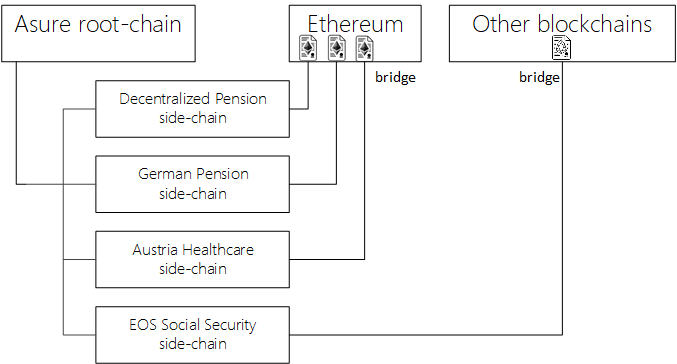
\includegraphics[width=4.0in]{img/chains.png}
    \caption{Сайдчейны Asure}
    \label{fig:asure_side_chains}
\end{figure}


%\newpage
\section{Asure Blockchain}
From a technical point of view social security systems can be described as a number of rule-based (financial) transactions which are executed between a (usually) slightly changing total of different parties under the condition to maintain an equilibrium between deposited and withdrawn value over a period of time. Such a system can be implemented digitally by creating a blockchain-system, which supports smart contracts and cryptocurrencies.

Conventional social security systems currently generate up to hundreds million transactions per month, depending on the number of parties involved and the specific social security use-case. 

\begin{table}[H]
\centering
\begin{tabular}{lp{.2\textwidth}l}
  Monthly pension premiums & = 54.445 Mio\\
  Monthly pensions & = 25.646 Mio\\\hline
  Monthly pension transactions & = 80.091 Mio
\end{tabular}
\caption{\label{tab:table-name} For example the German statutory pension system: \cite{eckzahlen}}
\end{table}

In order to develop a blockchain system that can process these transactions, it is necessary to increase the achievable transaction throughput of the system and automatic batch processing within a transaction to reduce the number of total transactions to a minimum.

Both requirements can be addressed by the use of side-chains, as specified in the Plasma Framework. The Asure Blockchain functions as the scalable side-chain of the Asure Plasma implementation. It is the root-chain of the Asure Network and lays the foundation for optimal scalability regarding blockchain-based social security systems. 

Assets transferred from the Ethereum Blockchain to one of the Asure side-chains, are locked up in the Asure Plasma Contract on the Ethereum Blockchain until an exit transaction on the Ethereum Blockchain is executed. According to the Plasma MVP specifications, an equivalent of this value is created through the use of the operator design pattern (Proof-Of-Authority) on the Asure Blockchain and assigned to the user.

The available assets on the Asure Blockchain can then be used for transactions within the system. Consensus between all node providers within the Asure Blockchain is reached through a proof-of-stake consensus algorithm by using an adapted version of the Tendermint consensus engine. \cite{tendermint} Tendermint can handle transaction volume up to 10,000 transactions per second. With the help of zones and sharding concepts, this size can be increased by a factor of 1000. This would ensure the sustainable operation of social security on blockchain. \cite{tendermint_bench}

\begin{figure}[H]
    \centering
    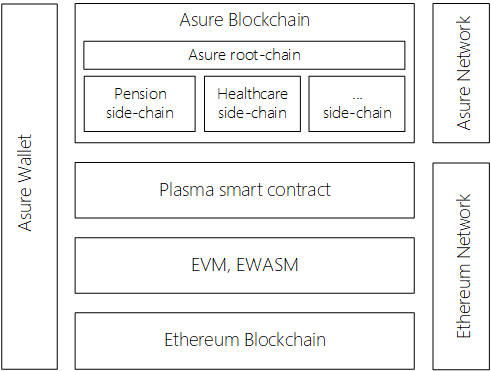
\includegraphics[width=4.0in]{img/architecture.png}
    \caption{Asure architecture}
    \label{fig:asure_architecture}
\end{figure}

The Asure Blockchain has several fundamentals. 

\subsection{Security}
The Asure Blockchain includes several features that protect it against such attacks as unauthorized spending, double spending, forging assets, and tampering with the blockchain. 

Each block added to the blockchain, starting with the block containing a particular transaction, is referred to as a confirmation of that transaction. Ideally, recipients and senders receiving payments should wait until at least one confirmation has been distributed across the network before assuming that the payment has been made. The more confirmations the recipient waits, the more difficult it is for an attacker to successfully reverse the transaction in a blockchain unless the attacker controls more than half of the total network performance, in which case it is called a 51\% attack. This construction is not designed to prevent 51\% of attacks, but rather to encourage block propagation. 

\subsection{Consensus algorithm}
There are different versions for proof algorithms. Proof-of-work is highly criticized because of enormous power consumption.\cite{hackernoon} Long-term acceptance and community movement is moving towards proof-of-stake where validators create the blocks and are rewarded for doing the correct job. The Asure blockchain will use a Proof-of-Stake (PoS) consensus algorithm. It will use in the first MVP implementation the Tendermint consensus engine.\cite{tendermint}

\subsection{Privacy with (ZK-SNARKS and ZK-STARK)}
Among other things, the Asure Blockchain takes into account privacy aspects that have an enormous relevance in relation to social security.

ZK-SNARKS (Zero-Knowledge Succinct Non-interactive Argument of Knowledge) offers the possibility to carry out anonymous transactions. The ZK-SNARKS are not resistant to Quantum Computing. ZK-STARK (Zero-Knowledge Scalable Transparent Argument of Knowledge) is the latest innovation aimed to achieve privacy on the blockchain with the use of fast, scalable computations and is resistant to Quantum Computing. \cite{iacr}

Since Ethereum is also researching in Layer 1 in this area, it will be possible for social security transactions to remain anonymous for those insured. \cite{ethereum_zksnarks}

The state of Zero-Knowledge technologies is not yet entirely practicable, but this will change in the future.

\subsection{EVM, WASM, eWASM, *WASM}
EVM provides a turing-complete computation so that Ethereum can run a general program, also known as a smart contract. Plasma EVM is a new version of Plasma that can execute EVM in plasma chain, and its clients can be based on current Ethereum clients (go-ethereum, py-evm, parity). We propose state-enforceable Plasma construction to guarantee only valid state submitted to root-chain, providing a way to enter and exit account storage between two chains because each chain has identical architecture. Another benefit is that Ethereum development tools can also be used in plasma chain.

eWASM is just an Ethereum "flavored" subset of Web Assembly, which is binary instruction format. eWASM  relies on instructions that are very close to real-world CPU. The performance improvements are significant and seem more secure. WebAssembly is backed by Mozilla, Google, Apple, and Microsoft, the community is also active, it's gonna be a widely used web standard.  

The Ethereum Blockchain processes about 15 transactions per second (TPS), which is not sufficient for the implementation of a social security system. The improvements to Ethereum (also called Layer 1), which are currently in progress, should significantly increase the number of TPS. Among the improvements are a Proof-of-Stake (PoS) based consensus algorithm, sharding, and by the introduction of eWASM - a WebAssembly based virtual machine.

\subsection{Further technologies}
Parity Substrate is a high-level framework for creating cryptocurrencies and other decentralized systems using the latest research in blockchain technology. 

Cosmos-SDK is a blockchain framework to allow developers to easily create custom interoperable blockchain applications within the Cosmos Network without having to recreate common blockchain functionality, thus removing the complexity of building a Tendermint ABCI application. We envision the SDK as the npm-like framework to build secure blockchain applications on top of Tendermint.

LotionJS aims to make writing new blockchains fast. It builds on top of Tendermint using the ABCI protocol. Lotion lets you write secure, scalable applications that can easily interoperate with other blockchains on the Cosmos Network.



\section{Asure Platform}

The Asure platform consists of components that provide the network and protocol for the use and construction of social security systems, including the Client, SDKs, tools and frontend applications. The purpose of the platform is to create an ecosystem in which social security systems can be developed, tested, simulated, managed and productively used as quickly as possible.

\subsection{Client}
Main client is the entry point into the Asure network, capable of running a node. Nodes are connected to each other in a peer-to-peer network and relay new information by gossip protocol. Each node keeps a complete copy of a totally ordered sequence of events in the Asure blockchain. The nodes are used to form and operate the Asure network and ensure that the transactions are included in the Asure blockchain.

\subsection{Software Development Kits (SDKs) }
The SDK provides standardized features on which applications can be built. Our primary goal is to simplify the development of new ecosystem solutions so that they require little to no developer support.

\subsection{Tools}
The tools support the creation, testing, and simulation of created solutions on the Asure network and blockchain and speed up the development process.

\subsection{Frontend applications}
In order to achieve user acceptance, the blockchain standard applications are provided, such as blockchain-explorer, pool, mobile-apps (Android, iOS,) with a wallet to make the experience of mobile payments on a  global scale possible, as well as unlocking the full potential of mobile commerce.


%\newpage

%
This document outlines important details about the upcoming ASR Token Generation Event (TGE), the purpose of the ASR token, and the legal requirements to participate in the ASR TGE.

\section{TGE}
The ASR TGE will happen in two rounds. The first round will take place at the beginning of 2019. The second round will happen later in 2019. Tokens will be ERC20 / ERC223 compatible and limited in supply by 100.000.000. In total, we will sell 45\% of all ASR utility tokens ("ASR") through the TGE.

\begin{table}[H]
\begin{tabular}{lp{.6\textwidth}l}
  Token name (Ticker) & Asure Token (ASR) \\  
  Token issuer & Asure Foundation, Zug, Switzerland\\
  Token type & ERC20 / ERC223 \\
  Total token supply & 100.000.000 ASR \\
  Token for sale & 45.000.000 ASR \\
  Accepted currencies & ETH \\
  Exchange Rate & 1 ASR = \$ 1.00 (ETH equivalent) \\
  Minimum Contribution & \$ 100 (ETH equivalent) \\\hline  
 
  Pre-Sale & tba 2019 \\
%19\textsuperscript{th} Feb - 12\textsuperscript{th} Mar 2019 \\
  Pre-Sale Cap & \$ 5.000.000 | 10 Million ASR\\
  Pre-Sale Terms & First week 40\% bonus\newline
                   Second week 30\% bonus\newline
                   Third week 20\%  bonus\\\hline
  
  Main-Sale & tba 2019 \\
%13\textsuperscript{th} Sep - 25\textsuperscript{th} Dec 2019 \\  
  Main-Sale Cap & \$ 35.000.000 | 35 Million ASR\\
  Main-Sale Terms & First month 15\% bonus\newline
                    Second month 5\% bonus\newline
                    Third month 0\% bonus\\\hline

%Special Bonus & 
%From \$ 5 to \$ 25 thousand  5\%\newline
%From \$ 25 thousand 10\%\\\hline

  Listing & ASR tokens will be listed on crypto exchanges \\

%Token Holder Benefits & 
%ASR token serves as the access to the Asure network by\newline
%\textbf{Network Validators:} Block rewards\newline
%\textbf{Service Providers:} Service rewards\\
%Token Trade Limitation & Only Team and Advisors have vesting and sales lock-in periods \\
  Hint & All unsold tokens in public TGE  will be burned \\\hline  
  
  Hardcap & \$ 40.000.000
  
\end{tabular}
\caption{\label{tab:table-name}Token details}
\end{table}

\section{Token}

The ASR token is a utility token. It is implemented as an Ethereum smart contract and supports the ERC-20 / ERC-223 token standards. The token will be used by Network Validators as well as Service Providers to participate as stakers in the proof-of-stake consensus mechanisms of the Asure network. It is an incentive to work correctly. Also, the ASR token will be used to govern the Asure network.

\begin{figure}[H]
    \centering
    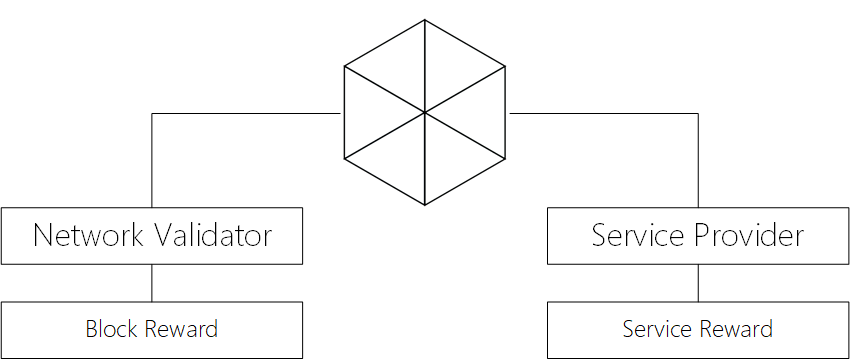
\includegraphics[width=4.0in]{img/staking.png}
    \caption{What Is Benefit For Our Token Holders}
    \label{fig:asure_architecture}
\end{figure}

\textbf{Network validators:}
Network validators need to stake a to be delivered amount of ASR tokens to validate transactions within the Asure network. In return, the network validators receive the networks transaction fees in the form of ASR as an incentive for validating correct blocks. In case of fraudulent behavior of a validator, the fraudulent validator will lose its stake to the network.

\textbf{Service providers:}
The ASR token serves as an incentive for service providers within the Asure platform to work correctly and as advertised within their SLA’s. Service providers must deposit ASR tokens which are retained in the event of non-compliance with the corresponding SLA. A service within the Asure network could be e.g. oracles, products, reinsurance, and sales activity.\newline

Demand for ASR tokens will be created by the two following mechanisms: With the growth of the Asure network and platform, more Network Validators and Service Providers will need to stake ASR tokens. The more Network Validators and Service Providers want to earn, the more ASR tokens must be staked.\newline
The ASR token will be listed on crypto exchanges for public trading so that service providers of the Asure Network, blockchain or platform can buy and sell ASR tokens.\newline

\textbf{Governance:}
On-Chain governance is crucial. ASR token holders will be able to govern the Asure blockchain, network, and vote over future improvements.
\newline\newline


\section{Token allocation}

It is very important that the community understands how Asure’s funds are going to be invested in the future in order to contribute to the idea of creating a world with an open decentralized autonomous system. See below how the investments will be allocated.

\begin{itemize}
\item \textbf{Phase 1:} 20\% of all ASR tokens will be generated.
\item \textbf{Phase 2:} 80\% of all ASR tokens will be generated.
\end{itemize}

\subsection{Phase 1}

In the first phase 20\% of all ASR token will be distributed.

\begin{table}[H]
\begin{tabular}{llp{.62\textwidth}l}
  10\% & Public Pre-Sale & Contributions will be used to develop the network minimal viable product, and to build bigger community.\\
  5\% & Family \& Friends & Family and Friends receive their tokens as part of their compensation package.\\
  5\% & Bounty & Asure provides compensation for a number of tasks spread across marketing, bug reporting or even improving aspects of the Asure network, blockchain and platform.
\end{tabular}
\caption{\label{tab:table-name} Phase 1 - Token allocation}
\end{table}

\subsection{Phase 2}

In the second phase 80\% of all ASR tokens will be distributed.

\begin{table}[H]
\begin{tabular}{llp{.62\textwidth}l}
  35\% & Public Main-Sale & Contributions will be used to develop the platform, and to fund security, legal and operational needs. \\
  35\% & Foundation & Comprises foundation development and education initiatives, incentives to developers and to research blockchain, scaling, network, and platform.\\
  8\% & Team  & These are placed to acknowledge the time, effort and resources contributed to the Asure platform.  The Asure team receive their tokens as part of their compensation package, and team tokens will be vested.\\
  2\% & Advisors & Advisors receive their tokens as part of their compensation package.
\end{tabular}
\caption{\label{tab:table-name} Phase 2 - Token allocation}
\end{table}

\subsection{Vesting}
According to best practice and in order to protect investors and future participants of our platform, we will lock up our team’s tokens. The Asure Team will receive their tokens in twelve equal parts over two years.
The vesting ensures token course stability and commitment of all involved team members. If a holder attempts to transfer more ASR tokens than vested, the transaction will be blocked.
We are going to publish the smart contract to control vesting within our project. Hence, we will prove to the community our long-term commitment.

\section{Funds allocation}

We envision that all ETH derived from the sale of ASR tokens will be allocated in the following manner:
\newline\newline


\begin{table}[H]
\begin{tabular}{llp{.6\textwidth}l}
  45\% & Platform R\&D & The creation of ongoing development of our Layer-2 network \\
  30\% & Marketing \& Operations & Additional staff and resources to cover day-to-day operations and prudent management as the organization expands. \\
  10\% & Legal & We are acutely aware of the need for rigorous compliance. We will need our own well-resourced legal support. Our principal concern is to fit within complex regulatory frameworks across the globe in order to make the growth of the community legally secure. \\
  10\% & Tax & Tax and organization development fees.\\
  5\% & Office Expenses & Office expenses and HR activities to build up
        a team to achieve roadmap goals
\end{tabular}
\caption{\label{tab:table-name}Funds allocation}
\end{table}

\section{KYC/AML}

The primary objective of token sale registration is to enforce a mandatory Know-Your-Customer (KYC) check to prevent identity theft, terrorist financing, Anti-money laundering (AML), and financial fraud. It also allows our team to understand our token holders better and manage risks appropriately.

The ASR tokens are not being offered or distributed to, as well as cannot be resold or otherwise alienated by their holders to citizens of, natural and legal persons, having their habitual residence, location or their seat of incorporation in the country or territory where transactions with digital coins are prohibited or in any manner restricted by applicable laws or regulations, or will become prohibited or restricted at any time after this agreement becomes effective (“Restricted Persons”).

We do not accept participation from the restricted persons and reserve the right to refuse or cancel the ASR token purchase requests at any time at our sole discretion when the information provided by the purchasers within the KYC procedure is not sufficient, inaccurate or misleading, or the purchaser is deemed to be a restricted person.

\section{Privacy and Security}
The security of your data is of great importance to us. There are no “cutting corners” when it comes to security, even under the pressure of running an ICO.  As such, please find below the measures which will be employed to ensure your privacy and security:

All your data will be stored in an encrypted form on our servers We don’t store your password as we only support external authentication providers like Google and Facebook All the information required for the KYC process will be wiped out from our systems once the checks are completed.

Asure will never share members’ personal data with 3rd parties without prior consent. In order to be on the safe side you should take these precautions:

Never send any fiat money or crypto coins to any address during the registration process. There is only one public token sale date and it is specified on our website: https://www.asure.network Bookmark the registration website, and never get to it following any email links.
Never trust emails related to the particular sale details (such as the information about soft or hard caps, Ethereum address to send to, etc.). Remember that a sender’s email address can be easily forged.
Never reply to our emails. Perform all your operations on our website only. You can check your registration status on our website using your account details.


\section{Excluded participants}
Due to legal restrictions citizens and residents from the following countries are not eligible to acquire ASR tokens: American Samoa, Belarus, Burundi, Central African Republic, Cuba, Congo (Brazzaville), Congo (Kinshasa), Guam, Iraq, Iran, Lebanon, Libya, Northern Mariana Islands, North Korea, Puerto Rico, Somalia, Sudan, South Sudan, Syria, United States, US Virgin Islands, US Minor Outlying Islands, Venezuela, Yemen, Zimbabwe.


\section{Опыт работы}

Основным направлением деятельности Asure в сфере социального обеспечения является пенсионное страхование. В рамках продолжающегося исследования мы перенесли специфические аспекты немецкой пенсионной системы в блокчейн Ethereum. Основываясь как на нашем практическом опыте, так и на опыте, накопленном за годы работы в области страхования, мы разработали теоретическую основу функционирования децентрализованной пенсионной системы, а также практическую реализацию такой системы. 

\subsection{Исследования технологии блокчейн и автоматизации}

Технический директор Asure, Фабиан Рец (Fabian Raetz), в 2013 году провел исследовательский проект в Университете прикладной науки и искусства в Дортмунде, где проанализировал новые технологии блокчейна и их возможное приминение. \cite{fraetz}
\newline

В 2014 году небольшая команда во главе с Полом Мизелем (Paul Mizel) и Фабианом Райцем (Fabian Raetz) разработала собственную валюту, основанную на блокчейне в качестве доказательства концепции и проверила различные виды проблем блокчейна и экономические системы (монета NRJ). \cite{nrjcoin}
\newline

В конце 2015 года Paul Mizel создал команду в Киеве для инновационных проектов на основе ИИ «Insure Chat», «Insure Assistant» и «Insure Advisor». В результате были созданы полностью автоматизированные чат-боты для поддержки, управления заявками и других задач с уникальным механизмом обучения и подключением к социальным платформам, таким как Facebook, Telegram, Skype и другие.\newline
Технический стек: IBM Watson, Microsoft Bot Framework, MS Luis, .NET.
\newline
Используемые алгоритмы: интеллектуальный анализ текста, регрессионный анализ, SVM, нейронные сети.

\subsection{Немецкая пенсионная система}
Чтобы продемонстрировать потенциал социального обеспечения, основанного на блокчейне, Asure создал прототип, основанный на модели немецкой государственной пенсионной системы с выплатой пенсии по факту.
\newline\newline

Asure dApp станет эталонной реализацией для dApps, использующих блокчейн и платформу Asure.
\newline\newline
Это предоставит
\begin{itemize}
\item техническое технико-экономическое обоснование пенсионной системы Германии, внедренной на блокчейне Ethereum и протоколе / платформе Asure.
\item полная реализация кошелька.
\item обзор и управление вашими страховыми полисами.
\item страховой магазин, чтобы найти и купить страховые полисы.
\end{itemize}

Пожалуйста, попробуйте Asure dApp, который в настоящее время работает на тестовой сети Ethereum Rinkiby: https://dapp.asure.io

\subsection{Децентрализованная пенсионная система}

Чтобы продемонстрировать, что блокчейн может решать проблемы в глобальном масштабе, Asure также разработала прототип глобальной пенсионной системы, которая полностью децентрализована и следовательно, не принадлежит ни правительству, ни какой-либо страховой компании.

Это эксперимент в альфа-фазе, призванный показать, как можно улучшить системы социального обеспечения в будущем с помощью технологии блокчейн.

Идея состоит в том, чтобы внедрить пенсионную систему с оплатой по факту на блокчейне Ethereum. Участники платят свои взносы в ETH и получают токены ERC20 взамен. Никакие вклады не вкладываются в рынок капитала и, следовательно, проценты не начисляются. Вместо этого, оплаченные ETH используются непосредственно для выплаты невыплаченных пенсионных требований. Сколько пенсии будет выплачиваться, зависит от того, сколько пенсионных токенов имеет пенсионер, то есть сколько взносов он внес в систему.

Как правило, системы pay-as-you-go работают только потому, что штаты вводят обязательные системы социального обеспечения и таким образом, могут гарантировать стабильное количество участников и выплаты взносов. В децентрализованной пенсионной системе никто не может быть принужден к членству. Членство в Asure создает несколько стимулов, которые должны привести к массовому принятию.

В децентрализованной пенсионной системе, как и в классической, любой кто вносит больший вклад, получает более высокую пенсию. Долгосрочные выплаты также играют роль. Чем дольше осуществляются регулярные выплаты, тем дольше будет выплачиваться пенсия.

\begin{figure}[H]
    \centering
    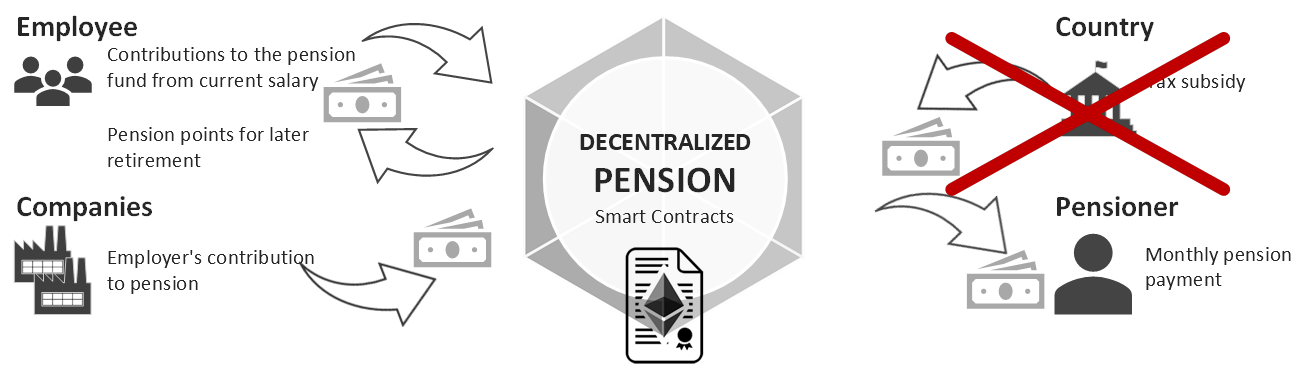
\includegraphics[width=5.0in]{img/pension.png}
    \caption{Модель PAYG}
    \label{fig:payg}
\end{figure}

В настоящее время децентрализованное пенсионное приложение Asure работает на тестовой сети Ethereum Rinkeby. Он был разработан во время ETHBerlin Hackathon и доступен по ссылке: 
\url{https://ethberlin.asure.io}

Пенсия это ставка, по которой сумма, которую я плачу, по меньшей мере так же велика, если не больше, чем выплата. Децентрализованная пенсия основана на немецкой пенсионной системе и имеет "генерационный контракт". Молодое поколение платит старшему поколению в соответствии со своими возможностями, а взамен пенсии распределяются по токенам в виде токенов пенсионных прав (PET).
\newline\newline

\subsubsection*{Модели стимулирования были разработаны в рамках проекта}
Система исключает управление возрастом, что позволяет избежать мошенничества. Время делится на периоды, где период - месяц. В течение каждого периода могут быть сделаны депозиты. Для каждого периода фиксированная целевая цена может измениться, если медиана депозитов предыдущего периода будет сильно отличаться от целевой цены. 

Если максимальное количество периодов было оплачено, также возможно максимальное количество пенсионных выплат. Предположим, что максимальное количество периодов равно 480 и равно 40 годам. Для ежемесячных выплат 40 лет, есть требование 40-летней пенсии. Если кто-то использовал систему только в течение 2 лет, заявка подана только на 1 месяц. Стимул к максимальному использованию системы вознаграждает участников с большим сроком пенсионного обеспечения.

\begin{eqnarray}
	entitlementMonths = \frac{payedMonths^2}{12 \cdot 40 years}
\end{eqnarray}

\begin{figure}[H]
    \centering
    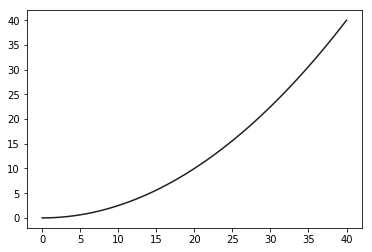
\includegraphics[width=3.0in]{img/pension_years.png}
    \caption{Децентрализованные пенсионные выплаты относительно получаемых лет}
    \label{fig:pension_years}
\end{figure}

Поскольку каждый может платить в системе разные суммы, максимальный плательщик получает максимальное двойное пенсионное право. Все те, кто платит больше, чем целевая цена периода, получат больше PET, но не более чем 2 за период. Максимально достижимые 960 PET, это позволит вам впоследствии претендовать на вдвое большее перераспределение, чем тот, кто активирует 480 PET.

\begin{eqnarray}
	DPT = \begin{cases} 1 + \frac{amount-amount_{max}}
	{targetPrice - amount_{max}} 
	* DTP_{bonus} & amount \geq targetPrice\\
	\frac{amount - amount_{min}}
	{targetPrice - amount_{min}} 
	* DTP_{bonus} & otherwise\end{cases}
\end{eqnarray}

\begin{eqnarray}
targetPrice - amount_{max} \neq 0 \quad and \quad targetPrice - amount_{min} \neq 0
\end{eqnarray}

В качестве дополнительного стимула для ранних пользователей в системе был предоставлен бонус, который имеет множитель 1.5, а время логарифмического приближения к 1.0 планируется приближать ежегодно.

\begin{eqnarray}
	DTP_{bonus} = f(year) = 1.5-0.12 * log(year)
\end{eqnarray}

\begin{figure}[H]
    \centering
    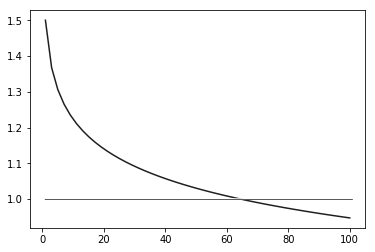
\includegraphics[width=3.0in]{img/pension_bonus.png}
    \caption{Децентрализованный пенсионный бонус по годам}
    \label{fig:pension_bonus}
\end{figure}

Если все выходят из системы, последние участники получают больше вознаграждений, поэтому мы гарантируем, что система останется прибыльной, поскольку нулевые участники системы снова будут установлены в исходное состояние.

Из-за ограничения в максимум 2 PET или с коэффициентом 1.5 первоначально 3 ПЭТ в течение периода в первые годы появляется возможность использования в системе нескольких счетов для оплаты, в которой система предотвращает передачу этих PET. 

С помощью этих стимулов и прозрачного дизайна и подхода DAO это начнется как социальный эксперимент после необходимых симуляций и корректировок параметров в сети Ethereum.

\subsubsection*{Преимущества}
Независимая крипто пенсия имеет много преимуществ, межпоколенческий контракт обеспечивает инфляционную безопасность. Он автономен и децентрализован в соответствии с идеей DAO. Там нет посредников. Конфиденциальность защищена, потому что никакие личные данные не нужны для участия в системе. Он полностью прозрачен, так как все транзакции находятся в блокчейне, а также с открытым исходным кодом.

\subsubsection*{Узнать больше}
Мы суммировали наши идеи о том, как основанная на перераспределении система взаимного пенсионного обеспечения могла бы выглядеть и поделились нашими результатами с более широким сообществом.
\newline
Depot Paper: \url{https://www.asure.network/asure.depot.en.pdf}



\newpage

\section{Дальнейшея работа}

Эта работа представляет собой единый путь к созданию сети Asure; Однако мы также считаем, что эта работа станет отправной точкой для будущих исследований децентрализованных систем социального обеспечения. В этом разделе мы определяем и заполняем две категории будущей работы. Это включает в себя работу, которая была завершена и просто ожидает описания и публикации и открытых вопросов для улучшения существующих протоколов.

\subsection{Текущая работа}

Следующие темы представляют текущую работу.

\begin{itemize}
\item Реализация Plasma MVP.
\item Мобильное приложение (Android, iOS)
\item Исследование децентрализованной системы социального обеспечения.
\item Контракты и протоколы интерфейса Asure-in-Ethereum.
\item Полная реализуемая спецификация протокола Asure.
\end{itemize}

\subsection{Открытые вопросы}
Есть еще области для улучшений, которые могут положительно повлиять на производительность сети. К ним можно вернуться позже после сбора достаточного количества статистических данных, по которым можно определить важность и необходимость внесения изменений:

\begin{itemize}
\item Лучшее решение для массовых стратегий входа и выхода.
\item Безопасное решение проблемы недоступности данных.
\item Более практическое применение SNARK/STARK.
\item Лучшая стратегия для более быстрого внедрения систем социального обеспечения и новых экономических моделей.
\item Лучший примитив для функции доказательства Proof-of-Stake, которая является публично-переменной и прозрачной.
\end{itemize}

Поскольку социальное обеспечение является лишь специализированной формой страхования, очевидно, что поддержка децентрализованного страхования на платформе также очевидна, и это хорошая пара для расширения этой платформы для рынка. Экосистема Asure состоит из сети Asure, протокола Asure, платформы Asure, на которой работают потенциальные сторонние приложения в области социального обеспечения и страховой среды. Признание экосистемы будет неуклонно расти из-за возникающих сетевых эффектов и синергии. 

\section{Организация}
Asure является некоммерческой организацией, основанной на трех основных принципах: инновации, сотрудничество и исследования с сообществом участников, занимающихся исследованиями и разработками для новых разработанных решений, созданных в сети Asure, блокчейном и платформой для разработки решений блокчейна с системами социального обеспечения и страхования в стиле DAO.
\newline

Организация включает в себя исследователей технологий, а также экспертов по страхованию. Asure является неотъемлемым компонентом нашей работы, который позволяет нам координировать взаимодействие в различных частях экосистемы.

\section{Благодарность}

Эта работа является совокупным усилием нескольких сотрудников команды Asure Foundation и не была бы возможна без помощи, комментариев и обзора соавторов и консультантов Asure Foundation. Мы также благодарим всех наших сотрудников и консультантов за полезные беседы; в частности, Andrey Kuchaev, Alexander Böhner, Dirk Mattern, Dennis Rittinghof, Michael Lurz, Emanuel Kuceradis и профессор доктор Hirsch.


\section{Summary}

This work had as its goal solving the listed problems with a decentralized approach as well as to show how a social security system can work in the future.

Thanks to public's voluntary participation, the invention of the incentives that makes the system a very interesting alternative became possible. A start for a transparent, fair and barrier-free pension that can be used worldwide.


If everyone adheres to the same rules, the only thing that occurs is that the system produces purchasing power. With 0\% inflation and 0\% deflation, the same number of $Units$ paid into the system will be paid out to users. Therefore there is no profit and no loss, but the value retention was simply being kept for years. \footnote{ The only costs incurred will be the transaction costs, in case of a private network, these can be further minimized.}

It is assumed that some users will opt for an earlier pension, even if it means partial loss for a user. Some users will lose full access to the system because e.g. the private key is lost, the pension contributions are not inherited and not collected. After some time, the paid-in values will be released, which will benefit the other users in the system.




\newpage

\listoftables

\listoffigures
 
\newpage
% Literaturliste endgueltig anzeigen
% \cite{ilo}
% NEW SITE ---------------------------------------------------------------------------------
\begin{thebibliography}{9}

  \bibitem{ilo}
  World social protection report 2017-2019,
   \textit{Universal social protection to achieve the sustainable development goals},
  International Labour Office, Geneva,
  2nd edition,
  2017.

  \bibitem{etherscan}
  Etherscan,
  \textit{Ethereum Transaction Chart},
  \url{https://etherscan.io/chart/tx},
  2017.

  \bibitem{worldometers}
  Worldometers,
  \textit{World Population Forecast (2020-2050)},
  \url{http://www.worldometers.info/world-population/},
  2017.  

  \bibitem{bitcoin}
  Satoshi Nakamoto,
  \textit{Bitcoin: A Peer-to-Peer Electronic Cash System},
  \url{https://bitcoin.org/bitcoin.pdf},
  2009.
  
  \bibitem{cammarden}
  Carmela Troncoso, Marios Isaakidis,George Danezis, Harry Halpin,
  \textit{Systematizing Decentralization and Privacy: Lessons from 15 Years of Research and Deployments, In Proceedings on Privacy Enhancing Technologies},
  De Gruyter Open,
  volume 2017,
  2017.

  
  \bibitem{gdpr}
  GDPR Info,
  \textit{General Data Protection Regulation},
  \url{https://gdpr-info.eu/},
  2018.  
  
  \bibitem{plasma}
  Joseph Poon and Vitalik Buterin, 
  \textit{Plasma: Scalable Autonomous Smart Contracts},
  \url{https://plasma.io/},
  2017.
  
 \bibitem{plasmamvp}
  Minimal Viable Plasma,
  \url{https://ethresear.ch/t/minimal-viable-plasma/426},
  2017.
  
  \bibitem{ethereum}
  Ethereum,
  \url{https://ethereum.org},
  2014.

  \bibitem{eckzahlen}
  Deutsche Rentenversicherung,
  \textit{Wichtige Eckzahlen},
  \url{https://www.deutsche-rentenversicherung.de/Allgemein/de/Navigation/6_Wir_ueber_uns/02_Fakten_und_Zahlen/03_statistiken/wichtige_eckzahlen_node.html},
  2016.

  \bibitem{hackernoon}
  Andrew Tayo,
  \textit{Proof of work, or proof of waste?},
  \url{https://hackernoon.com/proof-of-work-or-proof-of-waste-9c1710b7f025},
  2017.  
  
  \bibitem{tendermint}
  Jae Kwon,
  \textit{Tendermint: Consensus without Mining},
  \url{https://tendermint.com/static/docs/tendermint.pdf},
  2014.
  
  \bibitem{tendermint_bench}
  Zach,
  \textit{Tendermint: Benchmarks},
  \url{https://github.com/tendermint/tendermint/wiki/Benchmarks},
  2018.
  
  \bibitem{iacr}
  Eli Ben-Sasson, Iddo Bentov, Yinon Horesh, Michael Riabzev,
  \textit{Scalable, transparent, and post-quantum secure computational
integrity},
  \url{https://eprint.iacr.org/2018/046.pdf},
  2018.
  
  \bibitem{ethereum_zksnarks}
  Christian Reitwiessner,
  \textit{zkSNARKs in a nutshell},
  \url{http://chriseth.github.io/notes/articles/zksnarks/zksnarks.pdf},
  2016.

  \bibitem{fraetz}
  Fabian Raetz,
  \textit{Aufbau und Funktionsweise des Bitcoin-Protokolls},
  2014.  

  \bibitem{nrjcoin}
  NRJ Coin Project,
  \textit{NRJ Coin Project},
  \url{https://github.com/nrjcoin-project},
  2014.

  \bibitem{erd}
  European Report on Development (ERD): Deutsches Institut für Entwicklungspolitik,
  \url{https://www.die-gdi.de/erd/},
  2018.
  
  \bibitem{hcms}
  Health as Human Capital: Theory and Implications A New Management Paradigm, HCMS Group,
  \url{http://www.hcmsgroup.com/wp-content/uploads/2012/05/WP01-HHC-Theory-and-Implications-2012-01-161.pdf},
  2012.
 
  \bibitem{gaslimit}
  etherscan.io: gaslimit chart,
  \url{https://etherscan.io/chart/gaslimit},
  2012. 

\end{thebibliography}


\bibliographystyle{ieeetr}
%\bibliography{literatur}



\vskip 2.2in
\begin{quote}
	\centering
	Made with \ensuremath\heartsuit{ }in Germany 
\end{quote}

\end{document}
